\documentclass[tikz,border=12pt]{standalone}
% Shared visual language for standalone EMT block diagrams.
\usepackage{amsmath}
\usetikzlibrary{arrows.meta,backgrounds,calc,fit,positioning}

\tikzset{
    emt diagram/.style = {>={Stealth[length=2.4mm]}},
    line/.style        = {semithick, rounded corners=6pt},
    block/.style       = {draw, semithick, fill=white,
                          minimum height=1cm, minimum width=2.3cm},
    hblock/.style      = {block, minimum width=2.24cm, minimum height=1.3cm},
    vblock/.style      = {block, minimum width=1.3cm, minimum height=2.24cm},
    sum/.style         = {draw, semithick, fill=white, circle,
                          inner sep=2.6pt},
    signal/.style      = {circle, fill, inner sep=1.4pt,
                          label distance=3pt},
    sig/.style         = {font=\small},
    pm/.style          = {font=\scriptsize},
    wire jump/.style   = {line,
                          preaction={draw=white, line width=3pt,
                                     line cap=round}},
    enclosure/.style   = {draw, dashed, semithick, rounded corners=4pt},
    operator enclosure/.style = {enclosure, inner xsep=7mm, inner ysep=6mm}
}


% TUNABLES: gain width and the row of the modulation output.
\def\gainwidth{1.35cm}
\def\modulationrow{-2.2}
\def\supplyrow{1.8}

\begin{document}
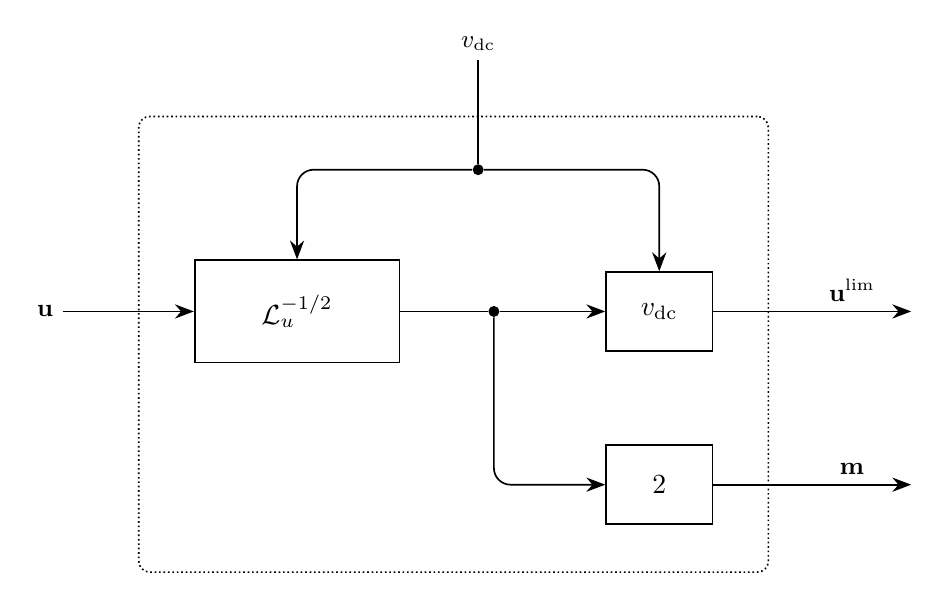
\begin{tikzpicture}[emt diagram]

% Radial limit of the voltage command against the available DC voltage.
\node[block, minimum width=2.6cm, minimum height=1.3cm]
    (limit) at (-1.6,0) {$\mathcal{L}_u^{-1/2}$};
\node[signal] (w) at (0.9,0) {};
\node[block, minimum width=\gainwidth] (dc) at (3,0) {$v_{\mathrm{dc}}$};
\node[block, minimum width=\gainwidth] (two)
    at (3,\modulationrow) {$2$};
\draw[line] (limit.east) -- (w);
\draw[->, line] (w) -- (dc.west);
\draw[->, line] (w) -- (0.9,\modulationrow) -- (two.west);

% Limited command returns to the current controller; the modulation
% command continues to the inverse Park transform.
\draw[->, line] (dc.east) -- node[sig, above, pos=0.7]
    {$\mathbf{u}^{\mathrm{lim}}$} (6.2,0);
\draw[->, line] (two.east) -- node[sig, above, pos=0.7]
    {$\mathbf{m}$} (6.2,\modulationrow);

% Voltage command and DC-link voltage inputs.
\node[sig] (u) at (-4.8,0) {$\mathbf{u}$};
\draw[->, line] (u.east) -- (limit.west);
\node[sig] (vdc) at (0.7,3.4) {$v_{\mathrm{dc}}$};
\node[signal] (vsplit) at (0.7,\supplyrow) {};
\draw[line] (vdc.south) -- (vsplit);
\draw[->, line] (vsplit) -- (-1.6,\supplyrow) -- (limit.north);
\draw[->, line] (vsplit) -- (3,\supplyrow) -- (dc.north);

% Enclose the operator.
\begin{scope}[on background layer]
    \node[operator enclosure, densely dotted,
        fit=(limit)(w)(dc)(two)(vsplit)] {};
\end{scope}

\end{tikzpicture}
\end{document}
